\chapter{Opis struktury projektu}
\label{chap:struktura_projektu}
Ten rozdział opisuje techniczną stronę projektu. Skupiam się w nim na użytych technologiach, architekturze oraz sposobie, w jaki zorganizowane są dane. Rozdział zamyka omówienie kluczowych klas i mechanizmów oraz wymagań niezbędnych do uruchomienia aplikacji.

\section{Wykorzystane technologie i narzędzia}
Sercem aplikacji jest język \textbf{Java}. To, co użytkownik widzi na ekranie, czyli interfejs graficzny, to zasługa biblioteki \textbf{Java Swing}. Wszystkie dane – o produktach, klientach czy zamówieniach – trafiają do bazy danych \textbf{MySQL}, a „mostem”, który łączy aplikację z bazą, jest technologia \textbf{JDBC}.

Nad całym kodem i historią jego zmian czuwał system kontroli wersji \textbf{Git}, a jego centralne repozytorium znajdowało się na platformie \textbf{GitHub}. Cały proces programowania odbywał się w środowisku \textbf{IntelliJ IDEA}. Aby ułatwić użytkownikowi wybieranie dat w kalendarzu, skorzystałem też z gotowej, zewnętrznej biblioteki \textbf{LGoodDatePicker} \cite{LGoodDatePicker}.

\section{Architektura i hierarchia klas}
Aplikacja ma przejrzystą budowę, ponieważ jest podzielona na trzy oddzielne warstwy. Każda z nich ma inne zadanie i nie miesza się z pozostałymi. Dzięki temu łatwiej jest zarządzać kodem i rozwijać program bez obawy, że zmiana w jednym miejscu zepsuje coś w innym.

\begin{enumerate}
    \item \textbf{Warstwa Prezentacji (View):} To po prostu wszystko to, co użytkownik widzi na ekranie i z czym może wejść w interakcję. Są to więc wszystkie okna, formularze i przyciski aplikacji, zdefiniowane w klasach takich jak \texttt{MainForm.java}, \texttt{AdminForm.java} czy \texttt{ShopRetailForm.java}.

    \item \textbf{Warstwa Logiki Biznesowej (Model):} To prawdziwe serce aplikacji – tu znajduje się cała „inteligencja” programu. Klasy w tej warstwie (np. \texttt{Product.java}, \texttt{Cart.java}, \texttt{Customer.java}) odwzorowują obiekty ze świata rzeczywistego i zawierają logikę ich działania, np. jak obliczyć sumę w koszyku czy jak dodać produkt.

\item \textbf{Warstwa Dostępu do Danych (Data Access Layer):} Ta warstwa to pośrednik, który zajmuje się wyłącznie komunikacją z bazą danych. Zastosowałem tu wzorzec \textbf{DAO}, aby zebrać w jednym miejscu cały kod odpowiedzialny za operacje na bazie. Dzięki temu reszta aplikacji nie musi przejmować się tym, jak dane są zapisywane i odczytywane, co upraszcza kod i czyni go bezpieczniejszym. Kluczowe metody, jak \texttt{OrderDAO.saveOrder()}, dbają o to, by operacje na bazie danych były bezpieczne i spójne.
\end{enumerate}
\clearpage

\subsection{Diagram klas UML}
Diagram klas (Rys. \ref{fig:uml_diagram}) to wizualna „mapa” projektu. Musiałem ją jednak znacznie uprościć. W aplikacji jest tak wiele klas i powiązań, że pokazanie wszystkich na raz stworzyłoby chaos, a nie czytelny obraz. Mimo to, diagram dobrze pokazuje podział na warstwy i najważniejsze zależności między nimi. Do jego wygenerowania użyłem narzędzia \textbf{PlantUML}, działającego jako wtyczka w IntelliJ IDEA.

\begin{figure}[H]
    \centering
    \includegraphics[width=1.1\linewidth]{figures/fig_0009.eps}
    \caption{Uproszczony diagram klas UML projektu.}
    \label{fig:uml_diagram}
    \small{Źródło: Opracowanie własne przy użyciu PlantUML}
\end{figure}
\clearpage

\section{Zarządzanie danymi i baza danych}
\label{sec:baza_danych_nowe}
Wszystkie informacje, z których korzysta aplikacja – dane o użytkownikach, produktach czy transakcjach – muszą być gdzieś trwale zapisane. Tę rolę pełni baza danych \textbf{MySQL}. Jej schemat (przedstawiony na \figurename~\ref{fig:erd_diagram}) pokazuje, jakie tabele przechowują poszczególne informacje i jak są one ze sobą powiązane. Główne grupy tabel odpowiadają za ewidencję użytkowników, katalog produktów, historię zamówień oraz finanse sklepu.

\begin{figure}[H]
    \centering
    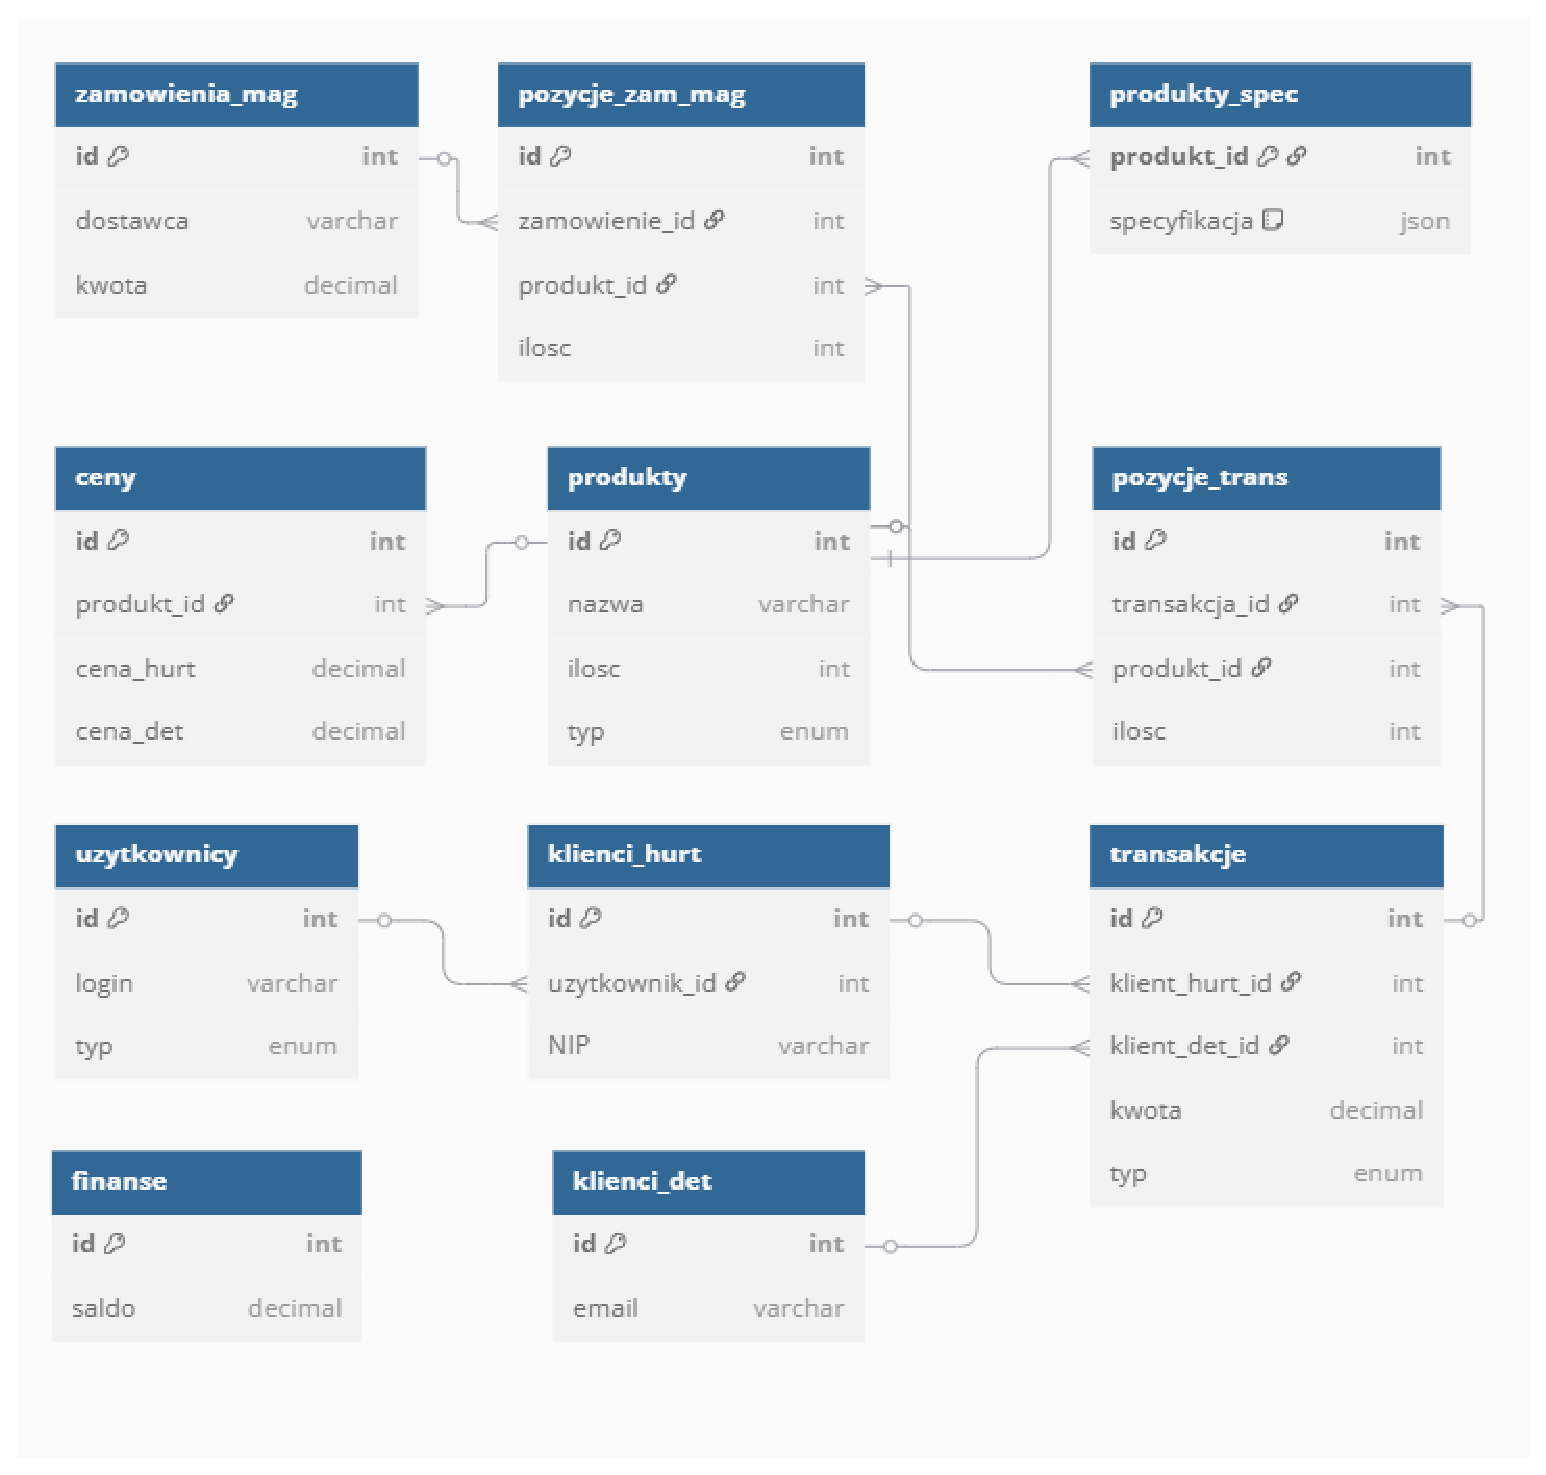
\includegraphics[width=\linewidth]{figures/fig_0001.eps}
    \caption{Schemat bazy danych (ERD) aplikacji sklepu.}
    \label{fig:erd_diagram}
    \small{Źródło: Wygenerowano za pomocą https://dbdiagram.io/}
\end{figure}
\clearpage

\section{Wymagania systemowe}
Aby uruchomić projekt na własnym komputerze i móc go rozwijać, potrzebne jest kilka darmowych narzędzi. Poniższa lista wyjaśnia, co i dlaczego należy zainstalować.
\begin{itemize}
    \item \textbf{Pakiet XAMPP:} To gotowy zestaw narzędzi, który w prosty sposób instaluje serwer bazy danych \textbf{MariaDB} (kompatybilny z MySQL). Jest on niezbędny, aby aplikacja miała gdzie przechowywać swoje dane.
    \item \textbf{Java Development Kit (JDK):} Jest to środowisko niezbędne do kompilowania i uruchamiania aplikacji napisanych w języku Java.
    \item \textbf{Środowisko IntelliJ IDEA:} To zaawansowany edytor kodu, w którym projekt był tworzony. Ułatwia on pracę z kodem, kompilację i uruchamianie programu.
\end{itemize}
Aktualne wymagania sprzętowe dla tych programów można znaleźć na ich oficjalnych stronach:
\begin{itemize}
    \item \textbf{XAMPP:} \url{https://www.apachefriends.org/download.html}
    \item \textbf{IntelliJ IDEA:} \url{https://www.jetbrains.com/help/idea/installation-guide.html#requirements}
\end{itemize}